\documentclass{standalone}
\usepackage{tikz,pgfplots}
\begin{document}
\resizebox{!}{\textheight - 3cm}{
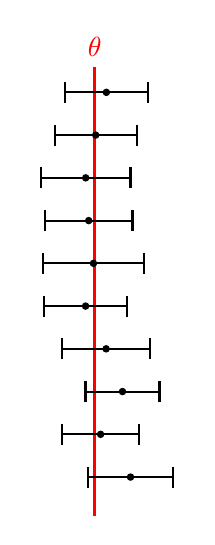
\begin{tikzpicture}[scale =1.9]
		\draw[red, line width = 1pt] (0,0)--(0,3) node[above]{$\theta$};
        \begin{axis}[
	    anchor=origin,  % Align the origins
	    x=1cm, y=1cm,   % Set the same unit vectors
	    hide axis
					]
\addplot+[only marks, color=black, mark options={fill=black, mark size = 0.5pt}, error bars/.cd, x dir=both,x explicit]
coordinates {
(0.238710797602868,0.285714285714286)+-(0.28682486688327,0.285714285714286)
(0.0386824372404836,0.571428571428571)+-(0.257098337836507,0.571428571428571)
(0.185228142705257,0.857142857142857)+-(0.247083029558065,0.857142857142857)
(0.0756553778851979,1.14285714285714)+-(0.292261999064447,1.14285714285714)
(-0.0614742041988502,1.42857142857143)+-(0.276784333071783,1.42857142857143)
(-0.0088265206506223,1.71428571428571)+-(0.335802592309207,1.71428571428571)
(-0.0406342399807429,2)+-(0.292927143761683,2)
(-0.0606789454935833,2.28571428571429)+-(0.299334368288613,2.28571428571429)
(0.00607251643980676,2.57142857142857)+-(0.273812480558445,2.57142857142857)
(0.0773351318055241,2.85714285714286)+-(0.277800783197014,2.85714285714286)
%(-0.239374418825707,3.14285714285714)+-(0.288244891971924,3.14285714285714)
%(0.240859231720267,3.42857142857143)+-(0.285336904040335,3.42857142857143)
%(-0.0534656394178079,3.71428571428571)+-(0.241728035216429,3.71428571428571)
%(-0.0990426029556093,4)+-(0.259881844237827,4)
%(0.146722506477234,4.28571428571429)+-(0.266443929722312,4.28571428571429)
%(-0.106241991207315,4.57142857142857)+-(0.293518250913707,4.57142857142857)
%(-0.0354998892616444,4.85714285714286)+-(0.241069955770645,4.85714285714286)
%(-0.311085365901295,5.14285714285714)+-(0.302588741508118,5.14285714285714)
%(0.0867208814353762,5.42857142857143)+-(0.274060836059998,5.42857142857143)
%(-0.0186966228452982,5.71428571428571)+-(0.271047817869804,5.71428571428571)

};

\end{axis}
\end{tikzpicture}
}

\end{document}